%%%%%%%%%%%%%%%%%%%%%%%%%%%%%%%%%%%%%%%%%%%%%%%%%%%%%%%%%%%%%%%%%%%%%%%%%%%%%%%%
%%%%%%%%%%%%%%%%%%   Vorlage für eine Abschlussarbeit   %%%%%%%%%%%%%%%%%%%%%%%%
%%%%%%%%%%%%%%%%%%%%%%%%%%%%%%%%%%%%%%%%%%%%%%%%%%%%%%%%%%%%%%%%%%%%%%%%%%%%%%%%

% Erstellt von Maximilian Nöthe, <maximilian.noethe@tu-dortmund.de>
% ausgelegt für lualatex und Biblatex mit biber

% Kompilieren mit
% latexmk --lualatex --output-directory=build thesis.tex
% oder einfach mit:
% make

\documentclass[
  tucolor,       % remove for less green,
  BCOR=12mm,     % 12mm binding corrections, adjust to fit your binding
  parskip=half,  % new paragraphs start with half line vertical space
  open=any,      % chapters start on both odd and even pages
  cleardoublepage=plain,  % no header/footer on blank pages
]{tudothesis}


% Warning, if another latex run is needed
\usepackage[aux]{rerunfilecheck}

% just list chapters and sections in the toc, not subsections or smaller
\setcounter{tocdepth}{1}

%------------------------------------------------------------------------------
%------------------------------ Fonts, Unicode, Language ----------------------
%------------------------------------------------------------------------------
\usepackage{fontspec}
\defaultfontfeatures{Ligatures=TeX}  % -- becomes en-dash etc.

% load english (for abstract) and ngerman language
% the main language has to come last
\usepackage[american, british]{babel}

% intelligent quotation marks, language and nesting sensitive
\usepackage[autostyle]{csquotes}

% microtypographical features, makes the text look nicer on the small scale
\usepackage{microtype}

%------------------------------------------------------------------------------
%------------------------ Math Packages and settings --------------------------
%------------------------------------------------------------------------------

\usepackage{amsmath}
\usepackage{amssymb}
\usepackage{mathtools}
\usepackage{braket}

% Enable Unicode-Math and follow the ISO-Standards for typesetting math
\usepackage[
  math-style=ISO,
  bold-style=ISO,
  sans-style=italic,
  nabla=upright,
  partial=upright,
  warnings-off={mathtools-colon,mathtools-overbracket}, % suppress some unnecessary warnings
]{unicode-math}
\setmathfont{Latin Modern Math}

% nice, small fracs for the text with \sfrac{}{}
\usepackage{xfrac}


%------------------------------------------------------------------------------
%---------------------------- Numbers and Units -------------------------------
%------------------------------------------------------------------------------

\usepackage[
  locale=DE,
  separate-uncertainty=true,
  per-mode=symbol-or-fraction,
]{siunitx}

%------------------------------------------------------------------------------
%-------------------------------- tables  -------------------------------------
%------------------------------------------------------------------------------

\usepackage{booktabs}       % \toprule, \midrule, \bottomrule, etc

%------------------------------------------------------------------------------
%-------------------------------- graphics -------------------------------------
%------------------------------------------------------------------------------

\usepackage{graphicx}
% currently broken
% \usepackage{grffile}

% allow figures to be placed in the running text by default:
\usepackage{scrhack}
\usepackage{float}
\floatplacement{figure}{htbp}
\floatplacement{table}{htbp}

% keep figures and tables in the section
\usepackage[section, below]{placeins}

% allows to include PDFs as full pages
\usepackage{pdfpages}

% Set the PDF Version of this document to 1.7 (1.4 is the current default)
% This is needed so that PDFs with Version >1.5 can be included
\pdfvariable minorversion=7

%------------------------------------------------------------------------------
%---------------------- customize list environments ---------------------------
%------------------------------------------------------------------------------

\usepackage{enumitem}

%------------------------------------------------------------------------------
%------------------------------ Bibliographie ---------------------------------
%------------------------------------------------------------------------------

\usepackage[
  backend=biber,   % use modern biber backend
  autolang=hyphen, % load hyphenation rules for if language of bibentry is not
                   % german, has to be loaded with \setotherlanguages
                   % in the references.bib use langid={en} for english sources
]{biblatex}
\addbibresource{references.bib}  % the bib file to use
\DefineBibliographyStrings{german}{andothers = {{et\,al\adddot}}}  % replace u.a. with et al.


% Last packages, do not change order or insert new packages after these ones
\usepackage[pdfusetitle, unicode, linkbordercolor=tugreen, citebordercolor=tugreen]{hyperref}
\usepackage{bookmark}
\usepackage[shortcuts]{extdash}

%------------------------------------------------------------------------------
%-------------------------    Angaben zur Arbeit   ----------------------------
%------------------------------------------------------------------------------

\author{Joel Koch}
\title{Key Experiments in Particle Physics}
\date{2024}
\chair{Experimental Physics IV}
\division{Faculty Physics}
% \thesisclass{Bachelor of Science}
% \submissiondate{29. Februar 2024}

% tu logo on top of the titlepage
\titlehead{
\includegraphics[height=1.5cm]{logos/tu-logo-eng.pdf}}

\begin{document}
\frontmatter
\maketitle  % Auskommentiert, da der Titel "Arbeit zum Erlangen des akademischen Grades..." entfernt wurde

\thispagestyle{plain}

\section*{Preface}

The summary of the course "Key Experiments of Particle Physics" from the winter semester of 2023/2024 will summarise one presentation from each session respectively.
It will be sorted not by the dates of the individual presentations but by the respective historical events.
The first chapter will be about semiconductors as they are used in the following experiments, except for the Wu experiment, and are thus a fundamental aspect of the detection of elementary particles.
The Wu experiment will be the second chapter being discussed, which provided the first experimental evidence for the violation of parity conservation in the weak interaction in 1956, leading to theoretical structures such as the $(V-A)$-structure and the CKM-Matrix and thus laying the foundation for particle physics.
The next chapter focuses on the discovery of the gluon in 1978, which took a significant step in the acceptance of the Standard Model of Particles (SM) \cite{Gaillard1998ui} as there had only been the photon discovered as one of the force-exchanging particles at the time \cite{DesyGluon}.
The last chapter will revise the oscillation of B-mesons ...
\tableofcontents

\mainmatter
% Hier beginnt der Inhalt mit Seite 1 in arabischen Ziffern
\chapter{Semiconductor Detectors}\label{Semiconductors}

The earliest studies of semiconductor detectors date back to 1833 when Faraday discovered the temperature dependence of the conductivity of silver sulphide.
Nearly a hundred years later, Wilson described a band theory of solids in 1931, in which quantum mechanics explains the characteristics of semiconductors.
The electrical conductivity can be described by the valence band (VB) which consists of positively charged quasiparticles that are called holes $h^+$ and the conduction band (CB) which is filled with electrons \cite{KolanoskiWermes}.
The band theory of solids distinguishes three types of conductive solids insulators with a band gap of $E_G\approx \SI{9}{\eV}$, with $E_G\approx \SI{1}{\eV}$ and conductors with no gap.
The properties of semiconductors can be changed by inserting impurities into the crystal structure.
If an atom with five electrons, called a donor, is inserted into an element with four electrons, an excessive conduction electron appears.
If an atom with three electrons, called an acceptor, is inserted into an element with three electrons, an excessive hole appears.
Semiconductors doped with donors are called n-doped while those doped with acceptors are called n-doped.
When both types of doped semiconductors are combined they form a diode.
Drifting and combining of $e^-/h^+$ forms an electrical field at the junction of the semiconductors which is called the depletion zone.
If an external positive voltage at the p side relative to the n side is applied this electrical field is weakened and current can flow which is called forward bias.
In reverse bias, the electrical field is strengthened and the depletion zone increases. 
This configuration is used in detectors to measure ionizing particles.
\begin{figure}[H]
    \centering
    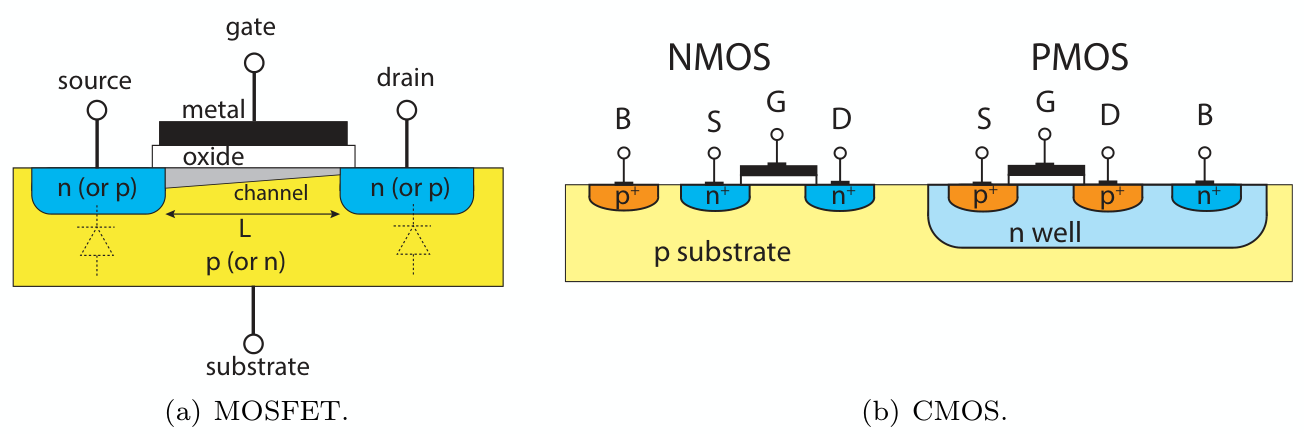
\includegraphics[width=0.69\textwidth]{figs/MOS.png}
    \caption{Schematic illustration of a MOSFET and a CMOS semiconductor \cite{KolanoskiWermes}.}
    \label{fig:MOStransition}
\end{figure}
The most used semiconductor detectors are complementary metal-oxide-semiconductors (CMOS) consisting of a part with a p-doped substrate and an n-doped drain terminal (NMOS) and a part with the reverse (PMOS).
Figure \ref{fig:MOStransition} a CMOS and a widely in field-effect transistor used semiconductor (MOSFET).

The simplest design of detectors is a pn area diode consisting of a $\SI{300}{\micro\meter}$ thick p and an n-doped area.
An additional guard ring can reduce the electrical noise.
Dividing the area into strips or pixels ($\text{length}<\SI{100}{\micro\meter}$) yields one or even two spatial coordinates but increases the readout difficulty.
There are two different types to read out the information from the collection diodes.
Hybrid pixel sensors have the readout electronics on a different chip which is a laborious assembly and resides in a large material thickness, the sensor, however, can be separately optimized to the readout components.
Monolithic pixel sensors reduce their material by an entire order of magnitude but not all production lines are suited to produce such sensors.
As pixel detectors are used to reconstruct traces for example in the ATLAS Experiment due to their good resolution with an uncertainty of $\sigma_x=\sfrac{\text{pitch}}{\sqrt{12}}$ \cite{Tom}, they are placed closest to the collision vertex where a lot of charged particles pass through them causing damage to the detector substrate.
Such radiation damage can cause a change in effective doping concentration leading to deactivated donor or acceptor atoms.
They can furthermore cause trapping where $e^-/h^+$ are trapped in defects of the crystal structure and are released later.
These defects can form energy levels that excite $e^-/h^+$ easier and cause a flow in current.
Radiation damage can be reduced by cooling \cite{Tom}.
\begin{wrapfigure}{l}{7.5cm}
    \centering
    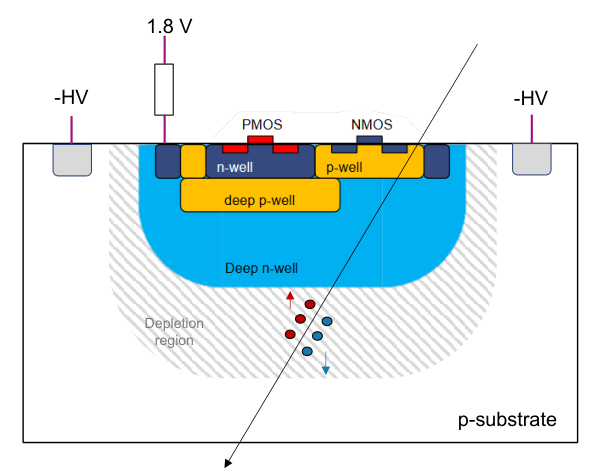
\includegraphics[width=0.5\textwidth]{figs/MightyPix.png}
    \caption{Schematic illustration of a MightyPix \cite{MightyPix}.}
    \label{fig:MightyPix}
\end{wrapfigure}
A track is reconstructed by forming groups of measurement points, called tracklets which require a good spatial and time resolution of the pixel detectors.
In each of the tracklets every possible combination is built but only those that point to the interacting point are accepted forming a track when a series of tracklets match.
An application of pixel detectors is given in the example of MightyPix, a design sketch of possible pixel detectors used in the second upgrade of the LHC.
Their final requirements for the upgrade include a time resolution of $<\SI{3}{\nano\second}$, and a pixel size of $~\SI{50}{\micro\meter}\times\SI{150}{\micro\meter}$.
Semiconductor detectors in the form of pixel detectors provide good time and space resolution which is why particle detectors are indispensable without them.
But the implementation of pixel detectors brings new challenges like the power distribution or the cooling of the detectors.

\chapter{Wu-experiment}
\label{cha:wu_exp}

The Wu experiment took place in 
\chapter{The Discovery of the Gluon}

In order to organize the vast amount of particles that have been discovered up to 1961 Murray Gell-Mann and Yuval Ne'eman proposed independently from each other the Eightfold Way.
The Eightfold Way organizes hadrons in dependence on the quantum variables strangeness and isospin. 
Mesons with a spin parity configuration of $0^-$ and baryons with a spin parity configuration of $\sfrac 12^+$ can both be organized in an octet.
Baryons with a spin parity configuration can be organized in a decuplet of which the tenth particle, the $\Omega^-(sss)$ has been proposed theoretically before it has been experimentally found later \cite{Fritzsch2018}.
The early quark model was proposed by Gell-Mann and George Zweig in 1964 which consisted of only the up-, down- and strange-quark.
An electron-proton scattering event from 1968 revealed partons that took up half of the carried momentum and were thus the first indication of gluons \cite{Venker}.
A theoretical description is given by Quantum Chromodynamics (QCD) after which the baryon wave function must be antisymmetric thus leading to the introduction of colour as another quantum variable that can be either red, green or blue.
QCD is a $\text{SU}(3)$ gauge symmetry theory that describes the strong interaction.
It predicts eight gluons as a gauge boson that can interact with itself.
Particles with a colour charge can never be detected as a single particle, because the energy to separate two particles increases until a particle-antiparticle pair is produced
Due to confinement, quarks and gluons combine with other colour-carrying particles forming new hadrons in a process called hadronisation.
These hadrons can in turn form new hadrons themselves building a cascade of particles called a jet.
The first evidence for jets was observed at the Stanford Positron Electron Asymmetric Rings (SPEAR) at $\SI{7.4}{\giga\eV}$ in 1975.
\chapter{Oscillation of neutral $B$-mesons}

The phenomenon of neutral mesons transforming into their respective antiparticle was first investigated by Gell-Main and Pais in 1955 \cite{PhysRev.97.1387}.
The CKM-matrix was introduced as an extension of the Cabbibo matrix in 1973 after discovering $CP$ violation which could not be explained with 4-quark-mixing \cite{10.1143/PTP.49.652}.
Each element of the matrix describes a transition between quark generations.
The neutral B meson $B^0_d(d\bar b)$ or respectively $B^0_s(s\bar d)$ can oscillate via two components, the on-shell $(E^2= p^2+m^2)$ and off-shell $(E^2\neq p^2+m^2)$ components.
Both are shown in \ref{fig:feynmanOnshell} and \ref{fig:feynmanOffshell} respectively.
\begin{figure}
    \centering
    \begin{subfigure}[B]{.5\textwidth}   % 1st subfigure
        \centering
        \includegraphics[width=.8\textwidth]{figs/feynmanOnshell.png}
        \caption{On-shell contribution.}
        \label{fig:feynmanOnshell}
    \end{subfigure}
    \begin{subfigure}[B]{.45\textwidth}   % 2nd subfigure
        \centering
        \includegraphics[width=.8\textwidth]{figs/feynmanOffshell.png}
        \caption{Off-shell contribution.}
        \label{fig:feynmanOffshell}
    \end{subfigure}
    \caption{Feynman diagram showing the neutral B meson oscillation \cite{Kpopp}.}
    \label{fig:feynmanDiagram}
\end{figure}
Measuring the oscillation frequency yields precise measurements of $V_{q_u b}$ and $V_{q_u d/s}$.
A time evolution can be deduced by introducing a mixing matrix in which non-diagonal elements occur due to oscillations via the box diagram \ref{fig:feynmanOnshell} and the on-shell contributions.
By diagonalising the mixing matrix an expression for the time evolution of flavour eigenstates can be found.
% Due to the on-shell contributions being much smaller than the off-shell contributions the oscillation frequency which results from a mass difference $\upDelta m_{d/s}$ is directly proportional to the matrix element $|V_{td}|^2$ resulting in an expression for the oscillation frequency
An expression for the oscillation frequency can be found due to the on-shell contribution being much smaller than the off-shell contributions $(\Gamma_{ij}<M_{ij})$ of $\upDelta m_{d/s}\propto |V_{td}|^2$ with $\upDelta m_{d/s}$ describing a mass difference \cite{artuso2019cp}.
The $B_d^0$ oscillation was first discovered at the ARGUS detector at DESY in 1987 \cite{ALBRECHT1987245}.
Earlier measurements were done by CLEO \cite{PhysRevLett.58.183}, MARK II \cite{SCHAAD1985188} and UA1 \cite{ALBAJAR1987247} collaborations.
Collisions of $e^+e^-$ at an energy of the $\Upsilon(4S)$ resonance produced $B^0_dB^0_d$ pairs which were used to measure the oscillation.
% Three analysis methods were used.
One of the methods to look for $B_d^0$ oscillation was to search for a fully reconstructed decay of $\Upsilon(4S)\rightarrow B^0_dB^0_d /\bar B^0_d\bar B^0_d$ which decayed flavourspecific via $B_d^0\rightarrow D^{*-}\pi^+/D^{*-}l^+\nu$ and  $\bar B_d^0\rightarrow D^{*+}\pi^-/D^{*+}l^-\nu$.
A different method was to reconstruct one $B_d^0$ from the $\Upsilon(4S)$ and tag the other $B_d^0$ with a lepton.
Using the same decay channels for the reconstruction of $B_d^0$ makes this method less sensitive to background originating from lepton misidentification.
It yielded a time-integrated oscillation parameter $r= \frac{\mathcal{BR}(B\rightarrow \bar B\rightarrow \bar X)}{\mathcal{BR}(B\rightarrow X)}$ of $r=\num{0.21(0.08)}$ which meant for the matrix element $V_{td}\neq 0$ \cite{ALBRECHT1987245}.

\begin{wrapfigure}{l}{5cm}
    \centering
    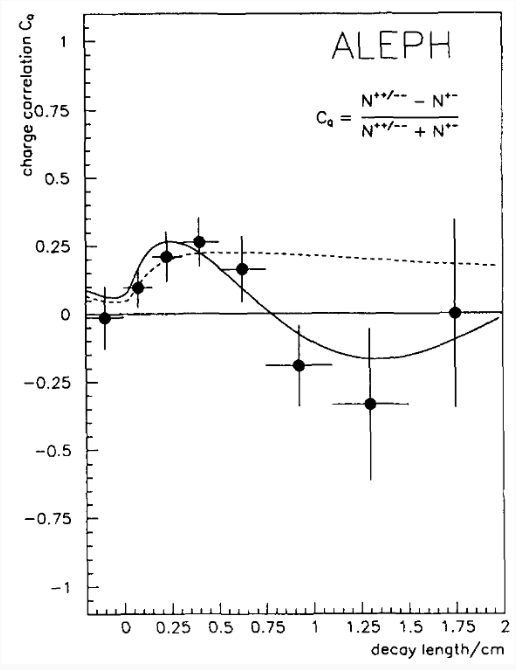
\includegraphics[width=0.3\textwidth]{figs/ALEPHresults.png}
    \caption{Fit to $Q_C(t)$ with a time dependent oscillation in data (solid) and a time independent approach (dashed) \cite{1993498}.}
    \label{fig:ALEPHresults}
\end{wrapfigure}
The ALEPH experiment at LEP measured the oscillation frequency $\upDelta m_d$ by tagging the state of $B_d^0$ at the time of production which decays semileptonic and at the time of decay which decays flavourspecific via $B_d^0\rightarrow D^{*-}X$ and $\bar B_d^0\rightarrow D^{*+}X$ \cite{1993498}.
Every \textit{correct} sign in the decay was defined as an unmixed event and vice versa by which a charge correlation function $C_Q(t)$ was defined.
At ALEPH the $B_d^0$ momentum was not reconstructed and the decay time was not calculated and only the decay length was used with boosting of $B_d^0$ that involved the momentum spectra.
Figure \ref{fig:ALEPHresults} shows an unbinned maximum likelihood fit to the decay length distribution to get $C_Q(t)$.
The involvement of the decay length distribution with the momentum spectra yielded the decay time.
An oscillation frequency of $\upDelta m_d = 0.52^{+0.10}_{-0.11}(\text{stat})^{+0.04}_{-0.05}(\text{syst})\, \text{ps}^{-1}$ was found \cite{1993498}.

\begin{wrapfigure}{l}{6.7cm}
    \centering
    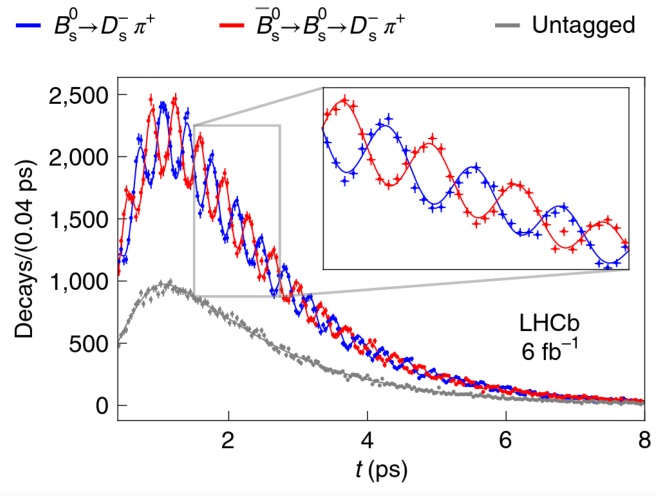
\includegraphics[width=0.48\textwidth]{figs/LHCbResults.png}
    \caption{Measurement of $B_s^0$ oscillations with the LHCb experiment \cite{LHCb2}.}
    \label{fig:LHCbResults}
\end{wrapfigure}
The oscillation of $B_s^0$ is more likely than the $B_d^0$ oscillation, due to $|V_{ts}|>|V_{td}|$ and was first discovered at CDF II in 2006 \cite{PhysRevLett.97.242003}.
Due to the mass difference of $s$ quarks being larger than those of $d$ quarks, a better time resolution was needed.
Measurements of $\upDelta m_d$ with the LHCb experiment at the LHC could increase the precision in 2016 \cite{LHCb1} to a value of $\upDelta m_d = 0.505\pm0.0021\,(\text{stat})\pm0.001\,(\text{syst})\,\text{ps}^{-1}$ leading to a matrix element of $V_{td}=\num{8.6(0.2)e-3}$ \cite{Workman:2022ynf}.
A study from 2022 found an oscillation frequency for $B_s^0$ of $\upDelta m_s = 17.7683 \pm 0.0051\,(\text{stat}) \pm 0.0032\,(\text{syst})\,\text{ps}^{-1}$ \cite{LHCb2} which lead to a value for the matrix element of $V_{ts}=\num{41.5(0.9)e-3}$ \cite{Workman:2022ynf}.
In figure \ref{fig:LHCbResults} the measurements of $B_s^0$ oscillations from the LHCb experiment are shown.
Figure \ref{fig:LHCbResults} shows the decay time of the $B_s^0\rightarrow D_s^-\pi^+$ signal decays are shown with the unmixed components shown in blue and the mixed components shown in red.

\appendix
% Hier beginnt der Anhang, nummeriert in lateinischen Buchstaben
% \input{content/a_anhang.tex}

\backmatter
\printbibliography

\cleardoublepage

\end{document}
